\section{扩展模型推导与结果图}

本附录保留正文中为控制篇幅而不逐项展开的推导、对照图与补充说明；正文中的结论、控制方程、题设要求表格及关键数值均不依赖本附录才能理解。

\subsection{节点中心有限体积离散}
在 $s\in[0,1]$ 上取节点 $s_i=i\Delta s$。以水分方程为例，界面通量为
\begin{equation}
G_{i+1/2}=s_{i+1/2}D_{i+1/2}\frac{C_{i+1}-C_i}{\Delta s},\qquad D_{i+1/2}=\tfrac12(D_i+D_{i+1}).
\end{equation}
内部、轴心和表面半控制体分别满足
\begin{align}
\Delta s\frac{\mathrm dC_i}{\mathrm dt}&=\frac4{R^2}(G_{i+1/2}-G_{i-1/2}),\\
\frac{\Delta s}{2}\frac{\mathrm dC_0}{\mathrm dt}&=\frac4{R^2}G_{1/2},\\
\frac{\Delta s}{2}\frac{\mathrm dC_N}{\mathrm dt}&=-\frac4{R^2}G_{N-1/2}-\frac{2h_m}{R}(C_N-W_{\mathrm{air}}).
\end{align}
温度方程仅将 $D,h_m,W_{\mathrm{air}}$ 依次替换为 $k,h,T_{\mathrm{air}}$，并保留 $\rho c_p$。节点中心半控制体使 Robin 通量直接装配，无需虚拟节点。

\begin{figure}[H]\centering
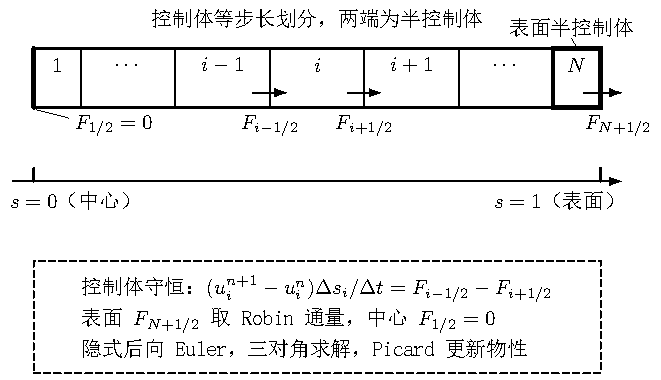
\includegraphics[width=.58\textwidth]{../figures/tikz_fv_stencil.pdf}
\caption{节点中心有限体积控制体与通量}\end{figure}

\subsection{问题一的扩展图与解析校验}
常物性温度方程的 Robin 特征函数为 $X_n=J_0(\zeta_n r/R_0)$，其中
\begin{equation}
\zeta_nJ_1(\zeta_n)=\mathrm{Bi}J_0(\zeta_n),\qquad \lambda_n=\alpha\zeta_n^2/R_0^2.
\end{equation}
令 $\theta=T-T_{\mathrm{air}}(t)$，则 $\dot b_n=-\lambda_nb_n-A_n\dot T_{\mathrm{air}}$；附件分段线性时逐段精确积分。该独立解与数值解的最大温度偏差为 $5.224\times10^{-4}$ °C。
\begin{figure}[H]\centering
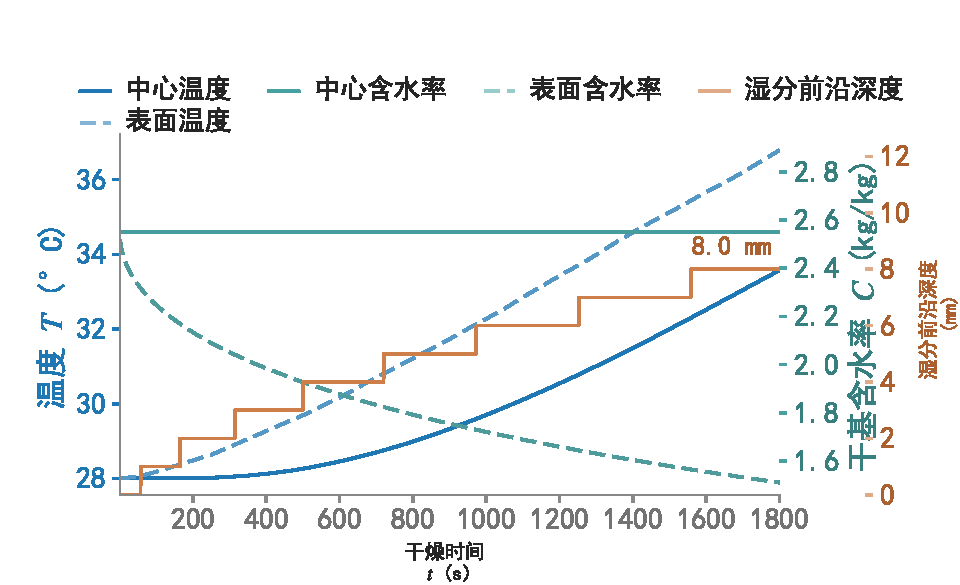
\includegraphics[width=.72\textwidth]{../figures/fig_q1_penetration.pdf}
\caption{问题一热湿推进对比}\end{figure}
\begin{figure}[H]\centering
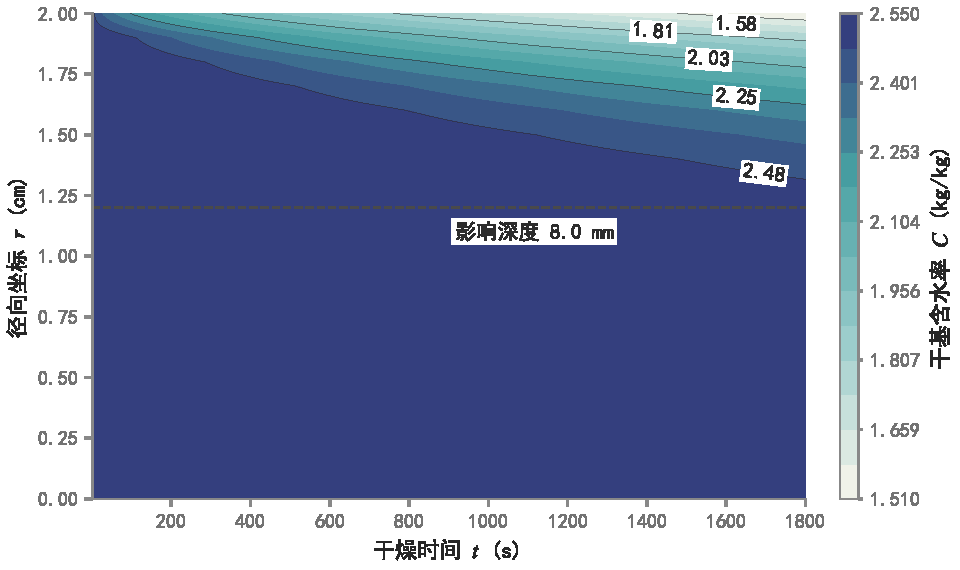
\includegraphics[width=.72\textwidth]{../figures/fig_q1_field_C.pdf}
\caption{问题一含水率场分布}\end{figure}
\begin{figure}[H]\centering
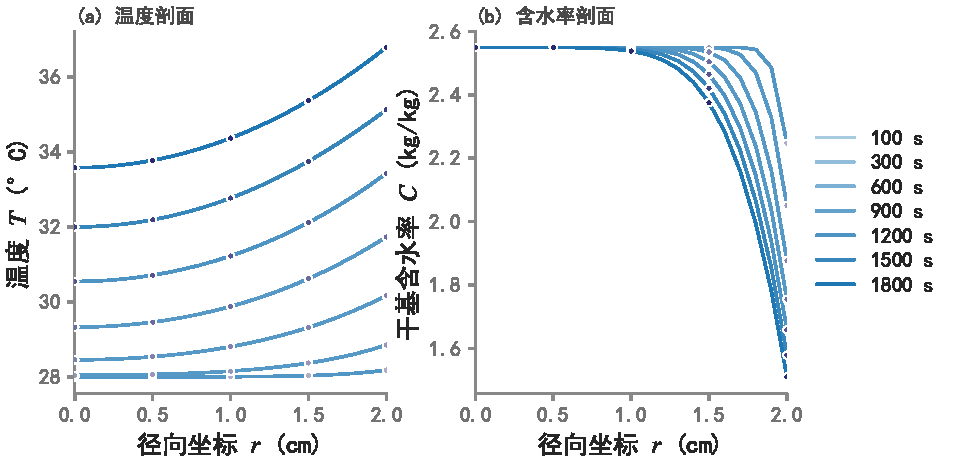
\includegraphics[width=.72\textwidth]{../figures/fig_q1_profiles.pdf}
\caption{问题一径向剖面族}\end{figure}
\begin{figure}[H]\centering
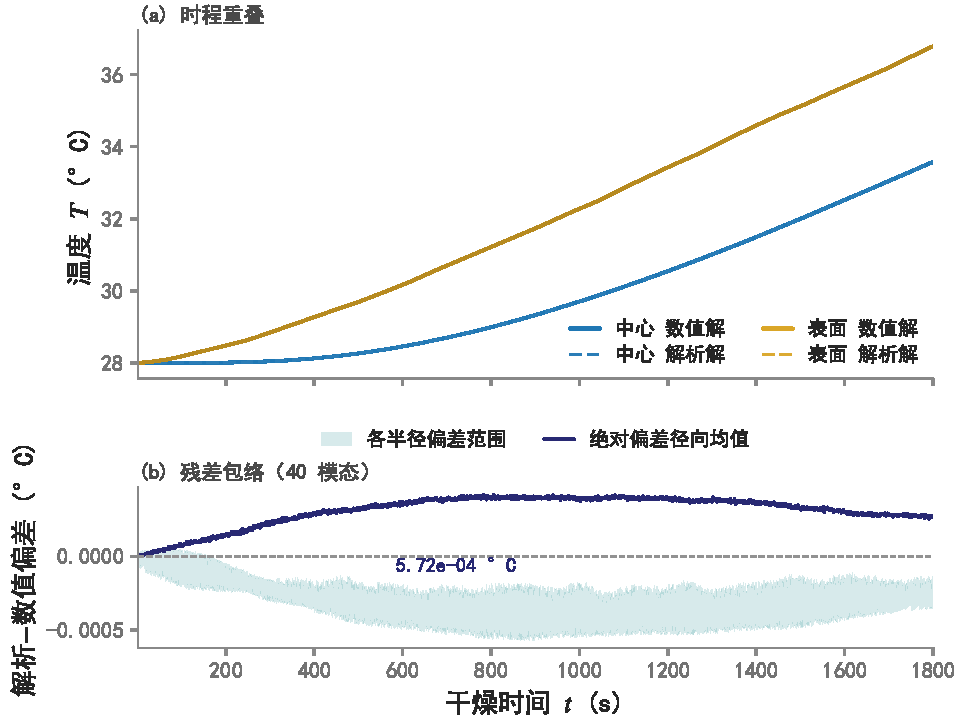
\includegraphics[width=.72\textwidth]{../figures/fig_q1_analytic_val.pdf}
\caption{问题一解析解与数值解完整对比}\label{fig:q1_analytic_val}\end{figure}

\subsection{问题二的扩展结果}
\begin{figure}[H]\centering
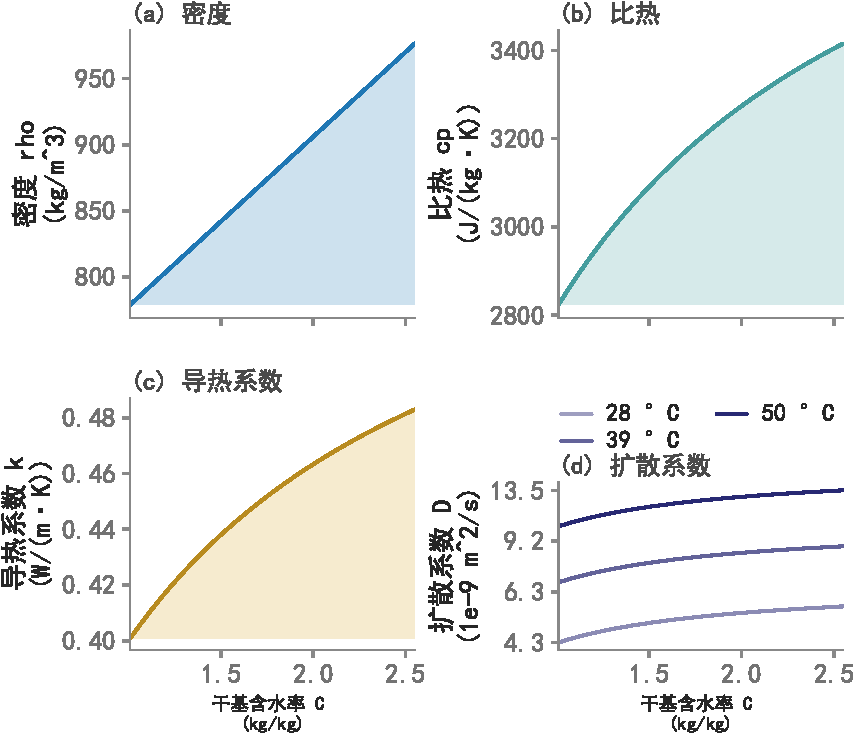
\includegraphics[width=.72\textwidth]{../figures/fig_q2_props_evolution.pdf}
\caption{附录三物性随含水率变化}\label{fig:q2_props_evolution}\end{figure}
\begin{figure}[H]\centering
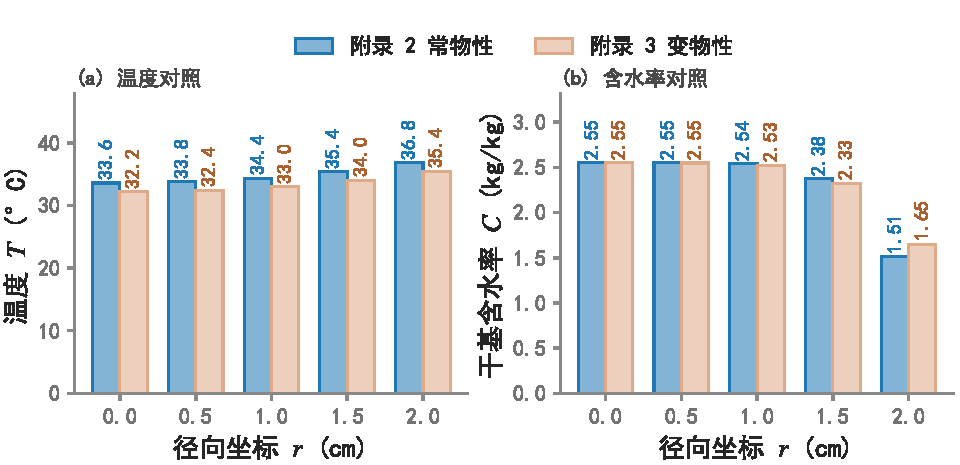
\includegraphics[width=.72\textwidth]{../figures/fig_q1q2_contrast.pdf}
\caption{常物性与变物性在 $1800$ s 的对照}\end{figure}
\begin{figure}[H]\centering
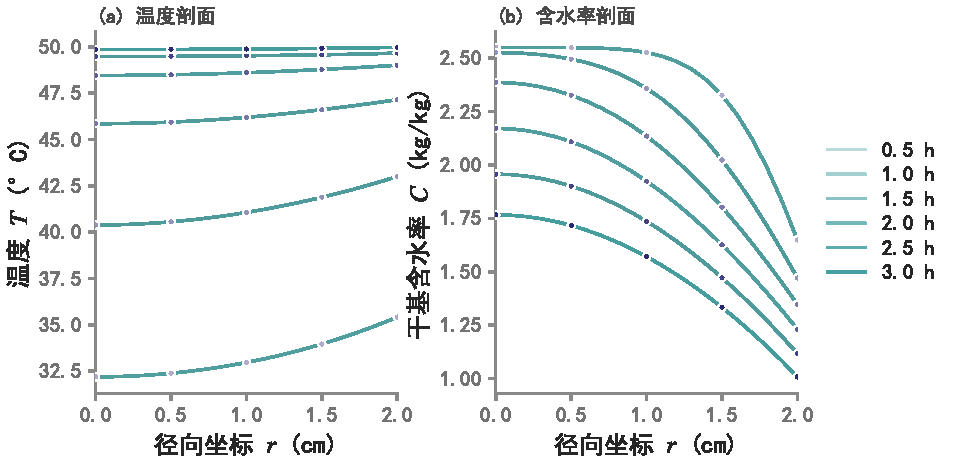
\includegraphics[width=.72\textwidth]{../figures/fig_q2_profiles.pdf}
\caption{问题二径向剖面族}\end{figure}

\subsection{问题四的扩展结果}
\begin{figure}[H]\centering
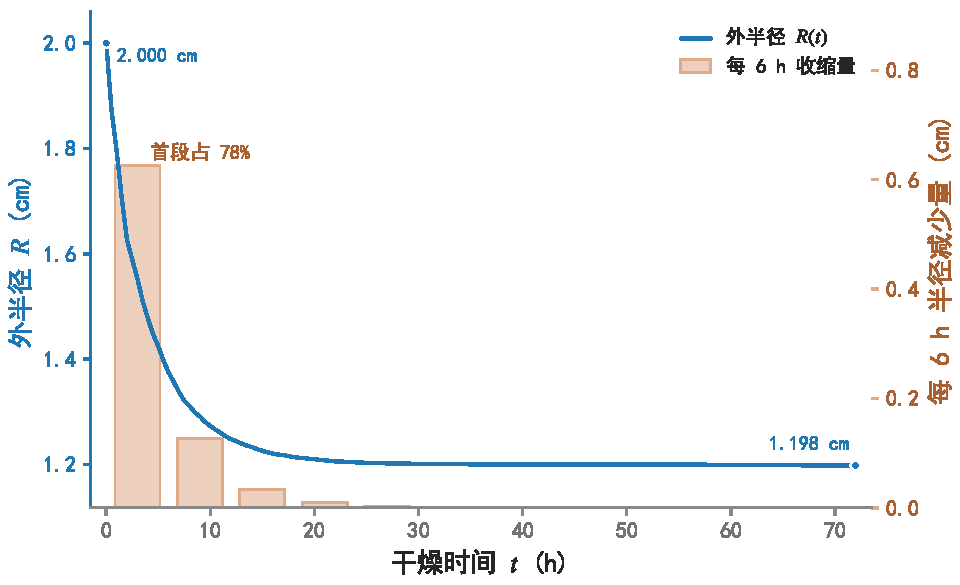
\includegraphics[width=.68\textwidth]{../figures/fig_shrinkage_curve.pdf}
\caption{药材半径收缩曲线}\end{figure}
\begin{figure}[H]\centering
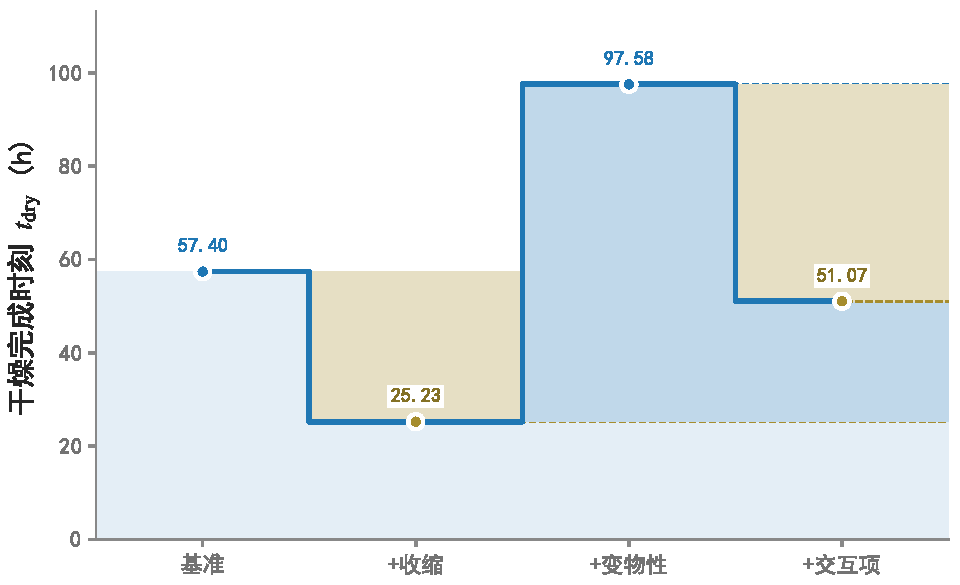
\includegraphics[width=.72\textwidth]{../figures/fig_q4_ablation.pdf}
\caption{收缩与物性的加性分解}\end{figure}
